\section{Introduction}
\label{section:introduction}

The present work is the final report for the Project Management module of the Degree's Final Project. This project will be carried out at the Barcelona School of Informatics and will be directed and supervised by Jordi Nin Guerrero, from the Computer Architecture department.

\subsection{Context summary}

Although a more thorough definition of the project's context will be given in section~\ref{section:context}, we will layout now the basics, in order to understand the scope and goals of the project.

\subsubsection{Data mining}
Today’s information society produces vast amounts of data all over the world. This data comes from innumerable sources and in diverse formats, and has been stored for years in data warehouses, waiting to be processed. Nowadays, all progress made in both hardware and software fields allows us to exploit this stored data and distill knowledge from it, through a series of techniques known as \textit{data mining}.\\

This is indeed a holistic process, where many different disciplines are involved, from data acquisition and storage, through its selection, filtering and analysis up to information extraction, visualization and knowledge discovery.\\

\begin{figure}[h]
	\centering
	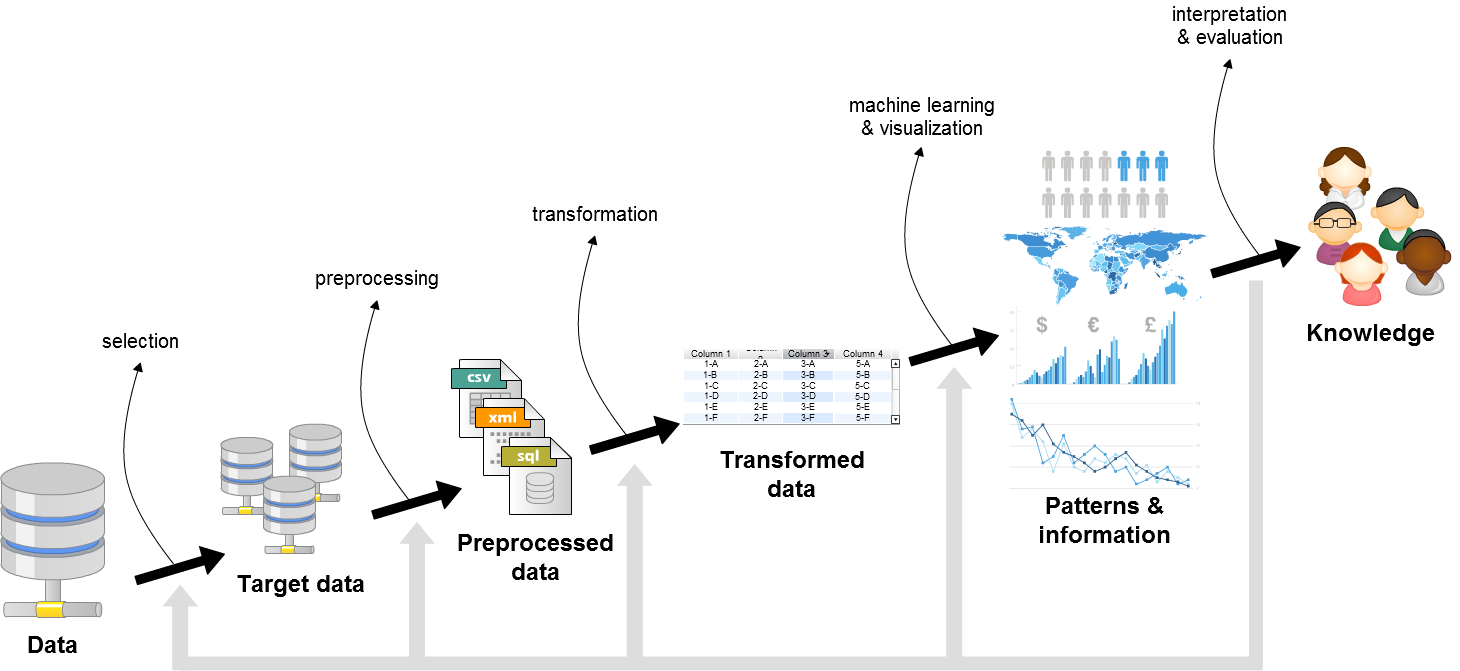
\includegraphics[width=0.9\linewidth]{figures/Untitled.png}
	\caption{Data mining as a process, from data acquisition to knowledge discovery. Source: adapted from \textit{From Data Mining to Knowledge Discovery in Databases}~\cite{Fayyad:1996:DMK:257938.257942}}
	\label{fig:data-mining}
\end{figure}


Data mining enables a better understanding of human or natural processes and provides us with means to identify trends, predict future events or discover useful patterns. Its uses range from scientific and medical applications to social sciences or business administration~\cite{Fayyad:1996:DMK:257938.257942}.\\

Despite lots of effort is put into enhancing different data mining processes, there still are many cases where these techniques fail to perform correctly; mainly, it is a matter of scale. On one hand, traditional data mining workflows cannot cope with the really massive data sets that are available nowadays, if performed on a common infrastructure. To solve this issue, clusters of hundreds or thousands of computers are used to run such analysis. It is costly and complex but, doing so, we can mine data that we couldn’t some time ago.\\

On the other hand, we face another type of scaling problem. In some situations, data acquisition throughput is so high that it can’t be stored anyway, so another approach is needed to avoid the loss of information that it could deliver us. Moreover, it could be that we didn’t want to store it, even when we could, but yet we wanted to analyze it to extract knowledge from it, as soon as we received it. Both scenarios are addressed with a series of techniques known as \textit{stream mining}.

\subsubsection{Stream mining}

Stream mining or data stream mining is a process that allows us to still discover knowledge and patterns in data, even when it comes in the form of a continuous stream, or many of them~\cite{Rajaraman:2011:MMD:2124405}. Instead of processing all statically stored data, like traditional data mining does, a relatively small portion of it is kept during the analysis, and it is updated when needed - either because more resources are available to the system or because new data is acquired.\\

MOA, initials for Massive Online Analysis, is an open source framework for data stream mining~\cite{website:MOA-Overview}, originally developed at the University of Waikato, New Zealand. It includes several machine learning algorithms\footnote{Algorithms used to perform the actual data mining analysis (the “machine learning \& visualization” step on figure~\ref{fig:data-mining}) belong to the field of machine learning. In MOA, clustering, classification, regression, outlier detection and recommender systems are available.}, to perform the analysis, tools to evaluate the quality of the results and also deals with a problem known as \textit{concept drift}\footnote{It is said of statistical properties of a target variable being analyed, when they change over time in unforeseen ways.}. It is related to the Weka\footnote{Weka is a popular software package including classical data mining algorithms, this is, not stream mining. It is also developed at the University of Waikato.~\cite{website:Weka}} package, but it is built to perform at a greater scale for more demanding problems.

\subsubsection{Privacy \& data mining}

Privacy has become a hot topic in debates nowadays, concerning what information is collected from individuals, who owns it and with which purposes. It is a matter of great importance and certainly worth to be examined carefully. Information technology brings us many benefits at many levels - safer streets, cheaper communications, better health systems, more convenient shopping - but at the high cost of losing our privacy.\\

Data mining is highly related to privacy. These knowledge discovery processes need data to work and, in most of the cases, it is sensitive personal data, which is massively gathered and stored and analyzed without us knowing much about it. Apart from the lack of consent in this data acquisition stage of the process, data mining poses a bigger thread on individuals: information disclosure.\\

A number of procedures have been developed to avoid information leaks at the individual level, while still being able to get knowledge from aggregated data. Different communities have worked on this area, which is called \textit{statistical disclosure control} by some or \textit{privacy preserving data mining} by others.


\subsection{The project in a nutshell}
\label{section:introductionNutshell}
Having presented its overall context, the main purpose of this project is to \textit{implement some privacy preserving data mining procedures within the MOA stream mining framework}. A more detailed description of the project is given in section~\ref{section:scope}.